\documentclass[11pt]{article}

\usepackage[margin=1.15in]{geometry}
\usepackage{amsmath, amssymb}
\usepackage{graphicx}
\usepackage{booktabs}
\usepackage{threeparttable}
\usepackage[expansion=false]{microtype}
\usepackage{setspace}
\usepackage[round]{natbib}
\usepackage[hidelinks]{hyperref}
\usepackage{caption}
\captionsetup{font=small, labelfont=bf, width=0.92\textwidth}

\graphicspath{{../figures/}}

\newcommand{\devig}{de-vigged}

\title{\textbf{Mispriced Tails, Cheap Fees, Uncertain Prices:\\
The Favorite--Longshot Bias in UFC Betting Markets\\
and Its Exploitability Net of Prediction-Market Costs}}
\author{Rawi Baransy\thanks{rawi.baransy@gmail.com. All results in this paper regenerate from a single
command (\texttt{python run\_analysis.py}) in the accompanying repository; see the Reproducibility
statement. This paper is a statistical study of historical prices and is not betting advice.}}
\date{August 24, 2026}

\begin{document}
\maketitle

\begin{abstract}
\noindent
We test whether mixed martial arts betting markets price fights efficiently, using 6{,}904 UFC bouts
from March 2010 to March 2026 with closing moneyline odds. Through the middle of the probability
range the market is strikingly well calibrated, and models built on public pre-fight statistics
cannot beat the closing line out of sample --- a semi-strong efficiency result. The tails, however,
are bent in the direction the favorite--longshot bias literature predicts: heavy underdogs win far
less often than their prices imply (bettors backing $+300$-or-longer underdogs lost 29 cents per
dollar staked, nearly nine times the bookmaker margin) and heavy favorites win more. A Mincer--Zarnowitz
calibration slope on \devig{} probabilities of 1.114 (fight-clustered SE 0.035) rejects efficiency
($p=0.001$), survives Shin's insider-trading correction ($1.068$, $p=0.046$), and strengthens over
time. Exploitability is a stricter claim: a favorites rule selected only on 2010--2017 data earned
$+1.9\%$ per bet out of sample on 975 bets in 2018--2026 --- beating the $-4.0\%$ efficient-market
benchmark --- but not statistically distinguishable from zero ($p=0.11$). We then price execution on
a regulated prediction market using Kalshi's official fee schedule, where the taker fee at
heavy-favorite prices is only $0.7$--$1.8\%$ of stake ($1.5\%$ at the sample's mean price). If the exchange mid tracks the \devig{}
sportsbook consensus, the same out-of-sample bets return $+4.5\%$ per bet ($p<0.001$), and remain
profitable across a one-cent half-spread ($+3.3\%$, $p=0.01$); the edge dies only if exchange prices
embed the bookmaker's margin ($+0.6\%$, $p=0.35$). Explicit trading costs are therefore not the
binding constraint on exploiting the anomaly --- price formation and liquidity are.
\end{abstract}

\section{Introduction}

When a betting market prices one fighter at $-800$ and the other at $+550$, do those prices still
reflect true win probabilities? For most of the probability range, betting markets are among the
best-calibrated forecasting institutions ever measured. But a persistent exception --- the
\emph{favorite--longshot bias} (FLB) --- has been documented for over seventy years, beginning with
horse racing \citep{griffith1949, ali1977, thaler1988}: longshots win less often than their prices
imply, favorites more often, so the expected return to backing longshots is far worse than the
bookmaker's margin alone can explain. Competing explanations divide into preference-based accounts
(risk-love or probability weighting by bettors) and belief-based accounts (systematic
misperception of small probabilities); \citet{snowberg2010} show field data favor the
misperception account. A separate supply-side mechanism is \citet{shin1993}: bookmakers shade
longshot prices to defend against insiders, generating FLB-like patterns even with unbiased
bettors --- which makes Shin's model the natural conservative benchmark when measuring the bias.

Mixed martial arts is a useful laboratory for three reasons. First, every bout is a two-outcome
contest with a single dominant bet type (the moneyline), so implied probabilities are clean and the
vig is measurable fight by fight. Second, the UFC posts an unusually wide range of prices ---
pick'ems through $-1500$ favorites --- so the tails are well populated. Third, MMA is young and
retail-heavy relative to the horse-racing markets of the classical literature, so it speaks to
whether FLB persists in a modern, high-attention sports market.

This paper makes three contributions. (i) It documents the FLB in UFC moneyline markets with
formal calibration tests and economic (returns-based) tests, under multiple vig-removal models and
with inference that respects the mirrored two-sides-per-fight structure of the data. (ii) It
separates \emph{bias} from \emph{exploitability} with a walk-forward protocol that selects a
betting rule on an early era and evaluates it blind on a later one, avoiding the data-snooping
critique that applies to full-sample strategy returns. (iii) It asks --- to our knowledge for the
first time in this literature --- whether the measured edge survives \emph{prediction-market}
execution costs, using the exact fee schedule of Kalshi, the largest CFTC-regulated event-contract
exchange, and explicit counterfactual assumptions about exchange price formation
\citep{wolfers2004, kalshifees}.

The answer to the exploitability question is sharp but conditional. At average sportsbook closing
prices the edge on heavy favorites beats the vig but does not clear zero with statistical
confidence. On an exchange, the relevant friction is not a margin inside the price but an explicit
fee that is \emph{smallest} exactly where the edge lives: Kalshi's taker fee of $0.07\,P(1-P)$ per
contract is $0.7$--$1.8\%$ of stake at heavy-favorite prices ($1.5\%$ at the sample's mean
price), versus roughly $4\%$ lost to the vig at a book. Under the standard assumption that a liquid exchange mid tracks the \devig{} book
consensus, the out-of-sample favorites rule returns $+4.5\%$ per bet ($p<0.001$) net of fees, and
$+3.3\%$ ($p=0.01$) after also crossing a one-cent half-spread. The result reverses only when the
assumed exchange price embeds the book's full margin. Fees, in short, are a rounding error on this
anomaly; the open question is what prices the exchange actually offers.

\section{Data}

The sample is the Ultimate UFC Dataset \citep{ufcdata}, which pairs every UFC bout with closing
American moneyline odds and pre-fight career statistics for both corners. After requiring
two-sided odds and a plausible book (overround between 1.00 and 1.25, which removes obvious
data-entry errors), the sample is 6{,}904 fights from 2010-03-21 to 2026-03-28. Draws and
no-contests (8 bouts, $<0.15\%$) are excluded from calibration and returns analysis; 6{,}896
decisive fights remain. The mean overround is $1.0355$, implying an efficient-market flat-bet
return of $1/r - 1 \approx -3.4\%$: a bettor facing fair \devig{} probabilities loses the vig and
nothing more. Clean public odds histories do not exist for other promotions (Bellator, PFL, ONE),
so the empirical sample is UFC; the pipeline is promotion-agnostic.

The unit of observation throughout is one \emph{side} of a fight --- one price a bettor could take
--- giving 13{,}792 sides. The two sides of a fight are mechanically mirrored (if one wins the
other loses), so no test in this paper treats them as independent: regressions cluster standard
errors by fight, bootstrap confidence intervals resample whole fights, and calibration buckets
de-duplicate fights whose two sides land in the same bucket.

\section{Empirical framework}

\subsection{From prices to probabilities}

American odds $a$ convert to decimal odds $d = 1 + a/100$ ($a>0$) or $d = 1 + 100/|a|$ ($a<0$),
and to raw implied probabilities $p = 1/d$. The two raw probabilities of a fight sum to the
booksum $r = p_A + p_B > 1$; $r-1$ is the bookmaker margin. Because raw probabilities embed the
margin, all calibration claims are stated for \devig{} probabilities under two models: (i)
\emph{proportional} normalization, $\pi_i = p_i / r$, the standard baseline under which the
flat-bet efficient-market return is the same $1/r - 1$ at every price --- the property that makes
return-by-odds-band comparisons interpretable; and (ii) \emph{Shin} (1993) probabilities, which
solve for the insider fraction $z$ per fight and shade longshots relative to proportional
scaling. Since Shin's model already attributes part of the raw FLB pattern to bookmaker
protection, any bias surviving Shin de-vigging is a conservative finding \citep{strumbelj2014}.

\subsection{Hypotheses}

The tests are organized as five pre-stated hypotheses.

\medskip
\noindent\textbf{H1 (Calibration).} De-vigged prices equal true win probabilities at every price
level. Test: Mincer--Zarnowitz on the logit scale \citep{mincer1969}, fitting
$\Pr(\text{win}) = \sigma\!\left(\alpha + \beta\,\mathrm{logit}(\pi)\right)$ by GLM with
fight-clustered standard errors; $H_0\!: \alpha=0, \beta=1$. $\beta > 1$ means outcomes are more
extreme than prices --- favorites underpriced, longshots overpriced (the FLB direction). As a
nonparametric complement, exact binomial tests per probability decile compare realized win rates
with mean implied probabilities, with Benjamini--Hochberg control of the false discovery rate
across buckets \citep{bh1995}.

\medskip
\noindent\textbf{H2 (Economic calibration).} The expected flat-bet return is $1/r-1$ at every
price. Tests: mean returns by American-odds band against the vig-only benchmark with
fight-cluster bootstrap intervals (4{,}000 resamples), and an OLS of per-bet return on implied
probability with fight-clustered standard errors, whose slope is zero under efficiency.

\medskip
\noindent\textbf{H3 (Semi-strong efficiency).} Closing prices impound public pre-fight
information. Test: models built from 17 public career differentials (record, physical attributes,
streaks, striking and grappling averages), fit on fights through 2021 and evaluated on 2022--2026,
must not beat the \devig{} market probability on out-of-sample log loss (paired bootstrap over
test fights). Fights are oriented favorite-vs-underdog so the arbitrary red/blue corner assignment
cannot leak, and features are computed directly from per-corner columns.

\medskip
\noindent\textbf{H4 (Exploitability at the book).} No rule committed to in advance earns
$\mathrm{ROI}>0$ at closing prices. Test: a walk-forward protocol. Eight favorite-cutoff rules
(bet every favorite at $-150$ or shorter, \dots, $-800$ or shorter) are evaluated on 2010--2017
only, one is selected by the \emph{most pessimistic} criterion (highest bootstrap lower confidence
bound, penalizing small lucky cells), and that single rule is staked blind on 2018--2026. Only the
out-of-sample numbers count as evidence.

\medskip
\noindent\textbf{H5 (Exploitability net of prediction-market costs).} The out-of-sample edge from
H4 does not survive realistic exchange execution. Test: reprice the same bets as event contracts
under Kalshi's official fee schedule \citep{kalshifees} --- taker fee $0.07\,C\,P(1-P)$, maker fee
$0.0175\,C\,P(1-P)$ per contract, charged on execution only, with free settlement --- under
explicit price-formation scenarios described in Section~\ref{sec:fees}.

\subsection{Inference conventions}

All confidence intervals for returns are percentile intervals from cluster bootstraps that
resample whole fights ($B=4{,}000$, fixed seeds); $p$-values for ROI are one-sided bootstrap
probabilities against $H_0\!:\mathrm{ROI} \le 0$ using the recentered bootstrap distribution.
Calibration regressions report cluster-robust (fight-level) standard errors. Because the \devig{}
probabilities of a fight's two sides are complementary by construction, the M--Z intercept is
mechanically zero for \devig{} columns and the slope test is the informative one-degree-of-freedom
statistic. No result in this paper depends on treating the 13{,}792 sides as independent
observations.

\section{Results}

\subsection{Calibration: efficient middle, bent tails (H1)}

Figure~\ref{fig:calibration} shows the calibration curve on \devig{} probabilities in probability
deciles with 95\% Wilson intervals. Through the middle of the range the market is nearly perfectly
calibrated: fights priced 30--70\% happen at almost exactly their implied rates (all deviations
$\le 1.3$ percentage points, none significant after FDR control). The tails bend in the FLB
direction. Sides priced 10--20\% (mean 16.3\%) won 12.8\% of 601 fights; sides priced 20--30\%
(mean 25.4\%) won 22.0\% of 1{,}616 (BH-adjusted $p = 0.009$). On the favorite side, prices of
70--80\% (mean 74.6\%) won 77.9\% of 1{,}622 (BH $p = 0.009$), and prices of 80--90\% (mean
83.7\%) won 87.6\% of 595 (BH $p = 0.035$). An equal-count robustness binning (27 quantile buckets
of roughly 500 bets each) bends identically at the tails.

\begin{figure}[t]
  \centering
  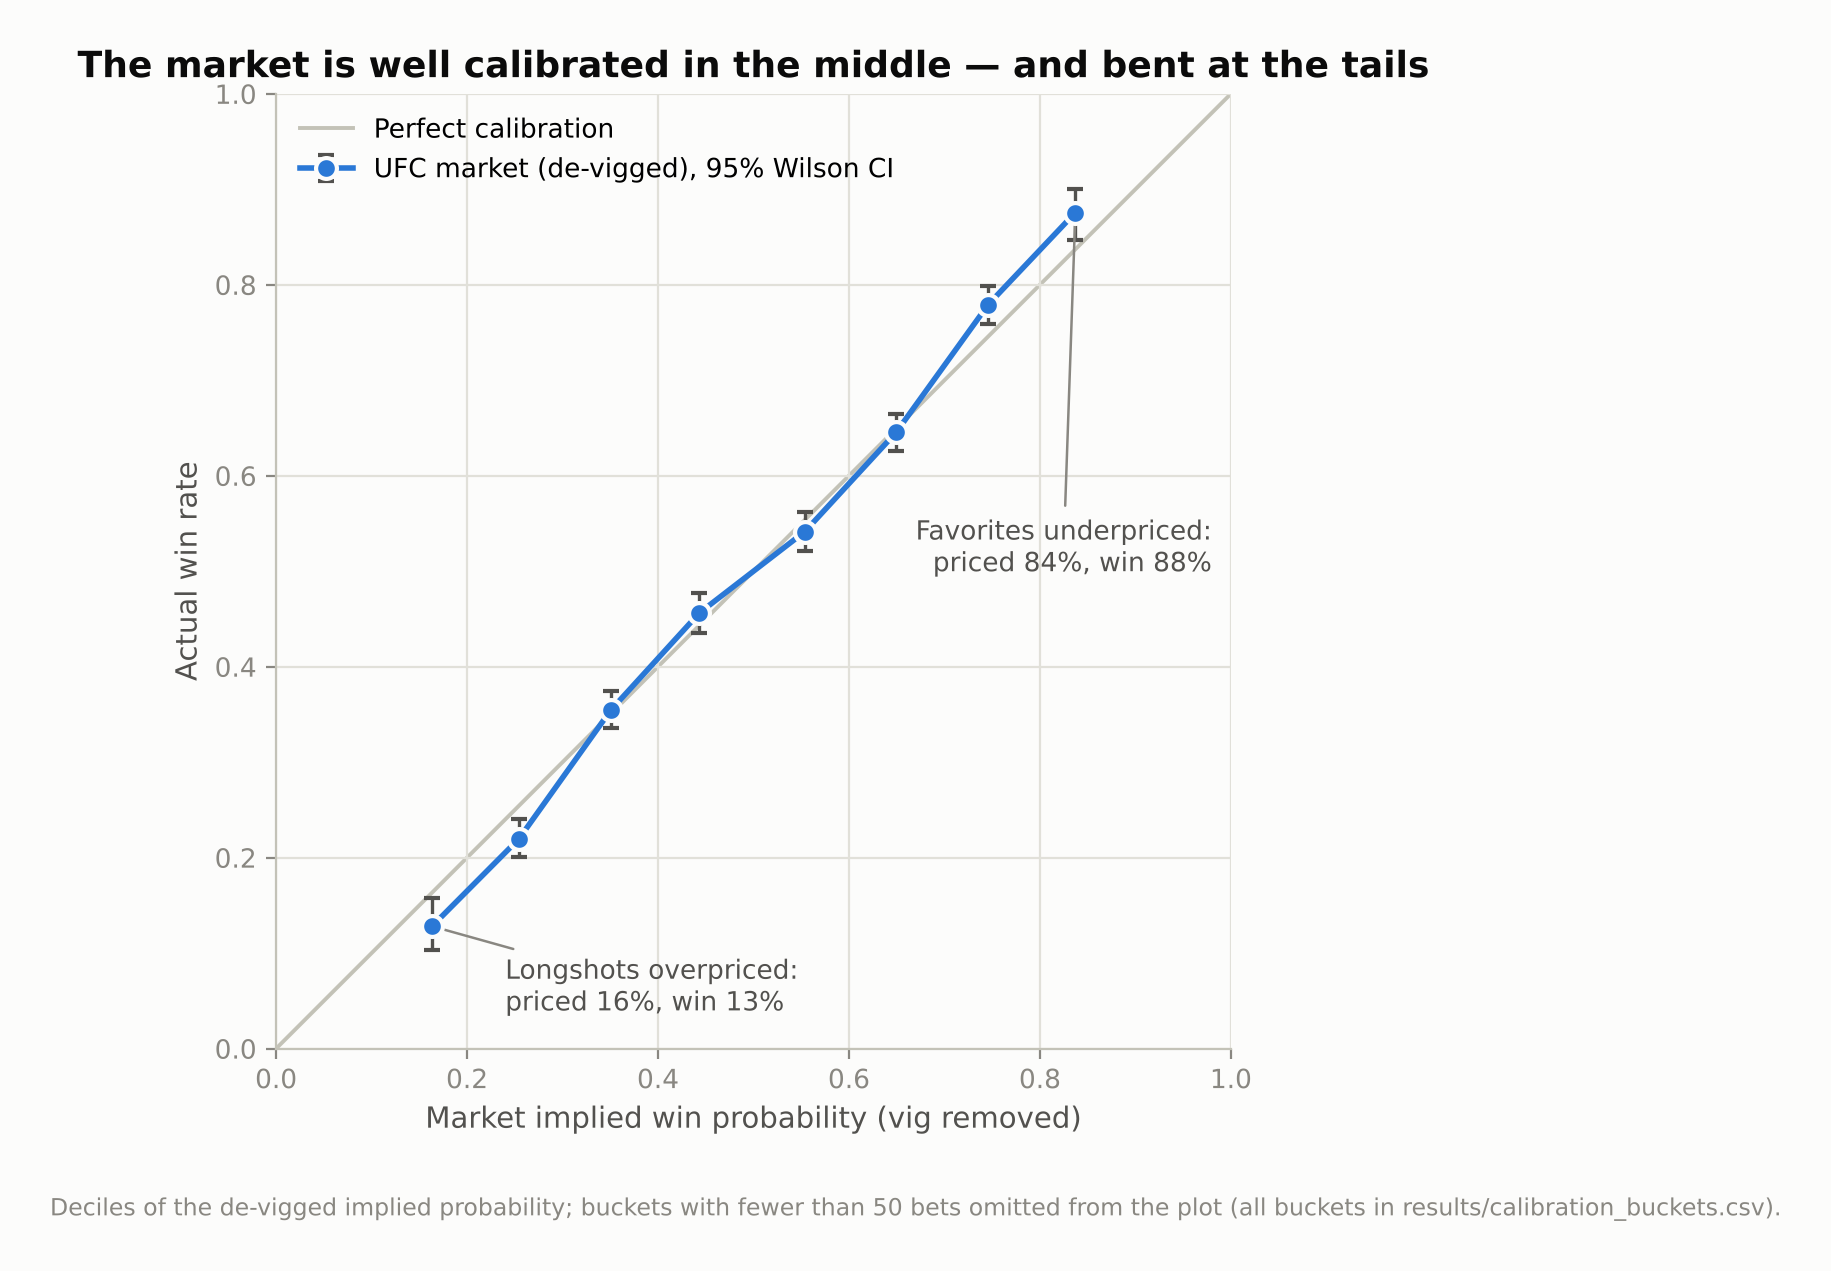
\includegraphics[width=0.78\textwidth]{calibration.png}
  \caption{Market calibration on \devig{} (proportional) implied probabilities, probability
  deciles, 95\% Wilson intervals. The market is nearly perfectly calibrated through the middle of
  the range and bent at both tails in the favorite--longshot direction.}
  \label{fig:calibration}
\end{figure}

Table~\ref{tab:mz} reports the formal test. On proportionally \devig{} probabilities the M--Z
slope is $1.114$ (SE $0.035$), rejecting $H_0\!:\beta=1$ at $p=0.001$. The estimate is above one
for raw probabilities as well ($1.063$, $p=0.061$; the margin itself masks part of the tail
distortion), and --- the conservative headline --- remains above one under Shin de-vigging
($1.068$, $p=0.046$). H1 is rejected: prices are too timid at the extremes even after allowing
for insider-defensive price shading.

\begin{table}[t]
\centering
\begin{threeparttable}
\caption{Mincer--Zarnowitz calibration tests, 13{,}792 sides of 6{,}896 fights.}
\label{tab:mz}
\begin{tabular}{lccc}
\toprule
Probability measure & Slope $\hat\beta$ & SE (fight-clustered) & $p$ for $H_0\!:\beta=1$ \\
\midrule
Raw implied ($p$)                 & 1.063 & 0.034 & 0.061 \\
De-vigged, proportional ($\pi$)   & 1.114 & 0.035 & 0.001 \\
De-vigged, Shin (1993)            & 1.068 & 0.034 & 0.046 \\
\bottomrule
\end{tabular}
\begin{tablenotes}\footnotesize
\item Logit-scale GLM $\Pr(\text{win}) = \sigma(\alpha + \beta\,\mathrm{logit}(\hat p))$.
$\beta>1$: outcomes more extreme than prices (favorites underpriced, longshots overpriced). For
\devig{} measures the intercept is zero by construction and the slope test carries the content.
\end{tablenotes}
\end{threeparttable}
\end{table}

\subsection{The economic version: returns by price (H2)}

Calibration gaps of a few probability points at the tails translate into enormous return
asymmetries because longshot payouts lever the error. Table~\ref{tab:bands} and
Figure~\ref{fig:bands} report mean flat-bet returns by odds band against the $-3.4\%$ vig-only
benchmark. Underdogs at $+300$ to $+499$ lost $26.8\%$ of stake per bet (95\% CI $[-37.4, -15.3]$,
$n=937$); underdogs at $+500$ or longer lost $37.0\%$ $[-59.7, -12.4]$ ($n=282$). No bookmaker
margin explains losing 27--37 cents per dollar when the margin is under four cents: this is
probability mispricing. On the other side, every favorite band from $-300$ on beats the
benchmark, and $-500$ to $-799$ favorites returned $+2.8\%$ $[-0.8, +6.5]$ against a $-3.5\%$
null (bootstrap $p = 0.002$ against the null). The OLS of per-bet return on implied probability
has slope $+0.258$ (fight-clustered $t = 3.76$, $p < 0.001$): every additional point of implied
probability raises expected return --- shorter prices are systematically better bets, the economic
signature of FLB. Cumulatively (Figure~\ref{fig:pnl}), flat-betting every $-300$-or-shorter
favorite over sixteen years ended $+26$ units on 1{,}804 bets \emph{through the vig}, while
flat-betting every $+300$-or-longer underdog lost 355 units on 1{,}219 bets.

\begin{table}[t]
\centering
\begin{threeparttable}
\caption{Flat-bet returns by American-odds band, 2010--2026.}
\label{tab:bands}
\begin{tabular}{lrrrrrc}
\toprule
Band & $n$ & Implied & Won & Return & 95\% CI & $p$ vs.\ vig null \\
     &     & (\devig{}) & & & & \\
\midrule
$-800$ or shorter & 175   & 0.877 & 0.909 & $-0.3\%$  & $[-5.2, +4.2]$   & 0.14 \\
$-799$ to $-500$  & 408   & 0.826 & 0.880 & $+2.8\%$  & $[-0.8, +6.5]$   & 0.002 \\
$-499$ to $-300$  & 1{,}221 & 0.759 & 0.795 & $+1.2\%$  & $[-1.6, +4.2]$   & 0.002 \\
$-299$ to $-200$  & 1{,}806 & 0.679 & 0.686 & $-2.5\%$  & $[-5.5, +0.6]$   & 0.53 \\
$-199$ to $-140$  & 2{,}050 & 0.600 & 0.585 & $-5.6\%$  & $[-8.9, -2.3]$   & 0.18 \\
$-139$ to $+99$   & 1{,}576 & 0.522 & 0.511 & $-5.9\%$  & $[-9.3, -2.6]$   & 0.24 \\
$+100$ to $+139$  & 1{,}746 & 0.443 & 0.458 & $-0.4\%$  & $[-5.5, +4.6]$   & 0.22 \\
$+140$ to $+199$  & 2{,}054 & 0.366 & 0.370 & $-2.5\%$  & $[-8.1, +3.2]$   & 0.76 \\
$+200$ to $+299$  & 1{,}537 & 0.286 & 0.281 & $-5.4\%$  & $[-13.0, +2.4]$  & 0.61 \\
$+300$ to $+499$  & 937   & 0.208 & 0.156 & $-26.8\%$ & $[-37.4, -15.3]$ & $<0.001$ \\
$+500$ or longer  & 282   & 0.135 & 0.089 & $-37.0\%$ & $[-59.7, -12.4]$ & 0.001 \\
\bottomrule
\end{tabular}
\begin{tablenotes}\footnotesize
\item One bet per listed price (both sides of every fight). CIs: fight-cluster bootstrap,
$B=4{,}000$. Vig-only null: $1/r - 1 \approx -3.4\%$ in every band under proportional margin;
$p$ is the two-sided bootstrap $p$-value against that null.
\end{tablenotes}
\end{threeparttable}
\end{table}

\begin{figure}[t]
  \centering
  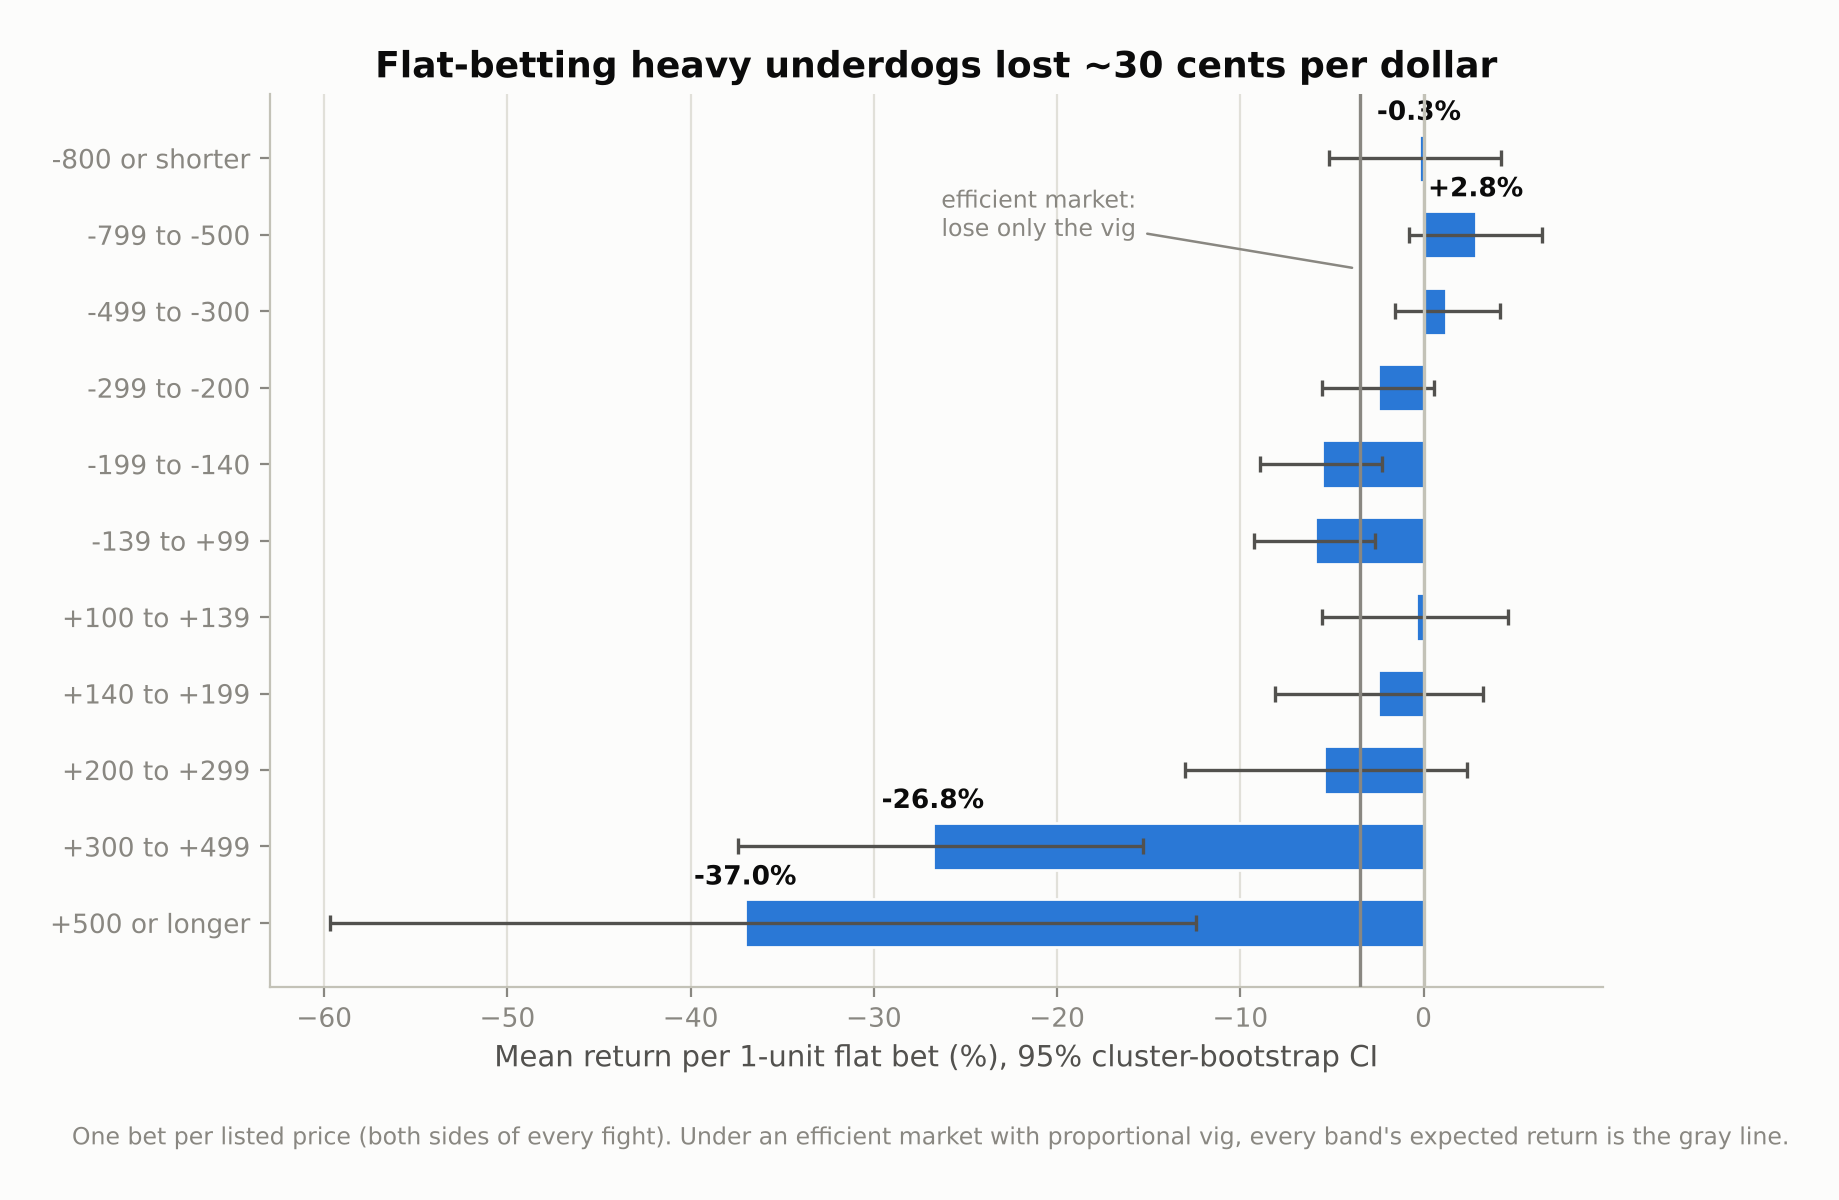
\includegraphics[width=0.9\textwidth]{returns_by_band.png}
  \caption{Mean return per 1-unit flat bet by odds band with 95\% cluster-bootstrap intervals.
  Under efficiency every band's expected return equals the vig-only benchmark (gray line).}
  \label{fig:bands}
\end{figure}

\begin{figure}[t]
  \centering
  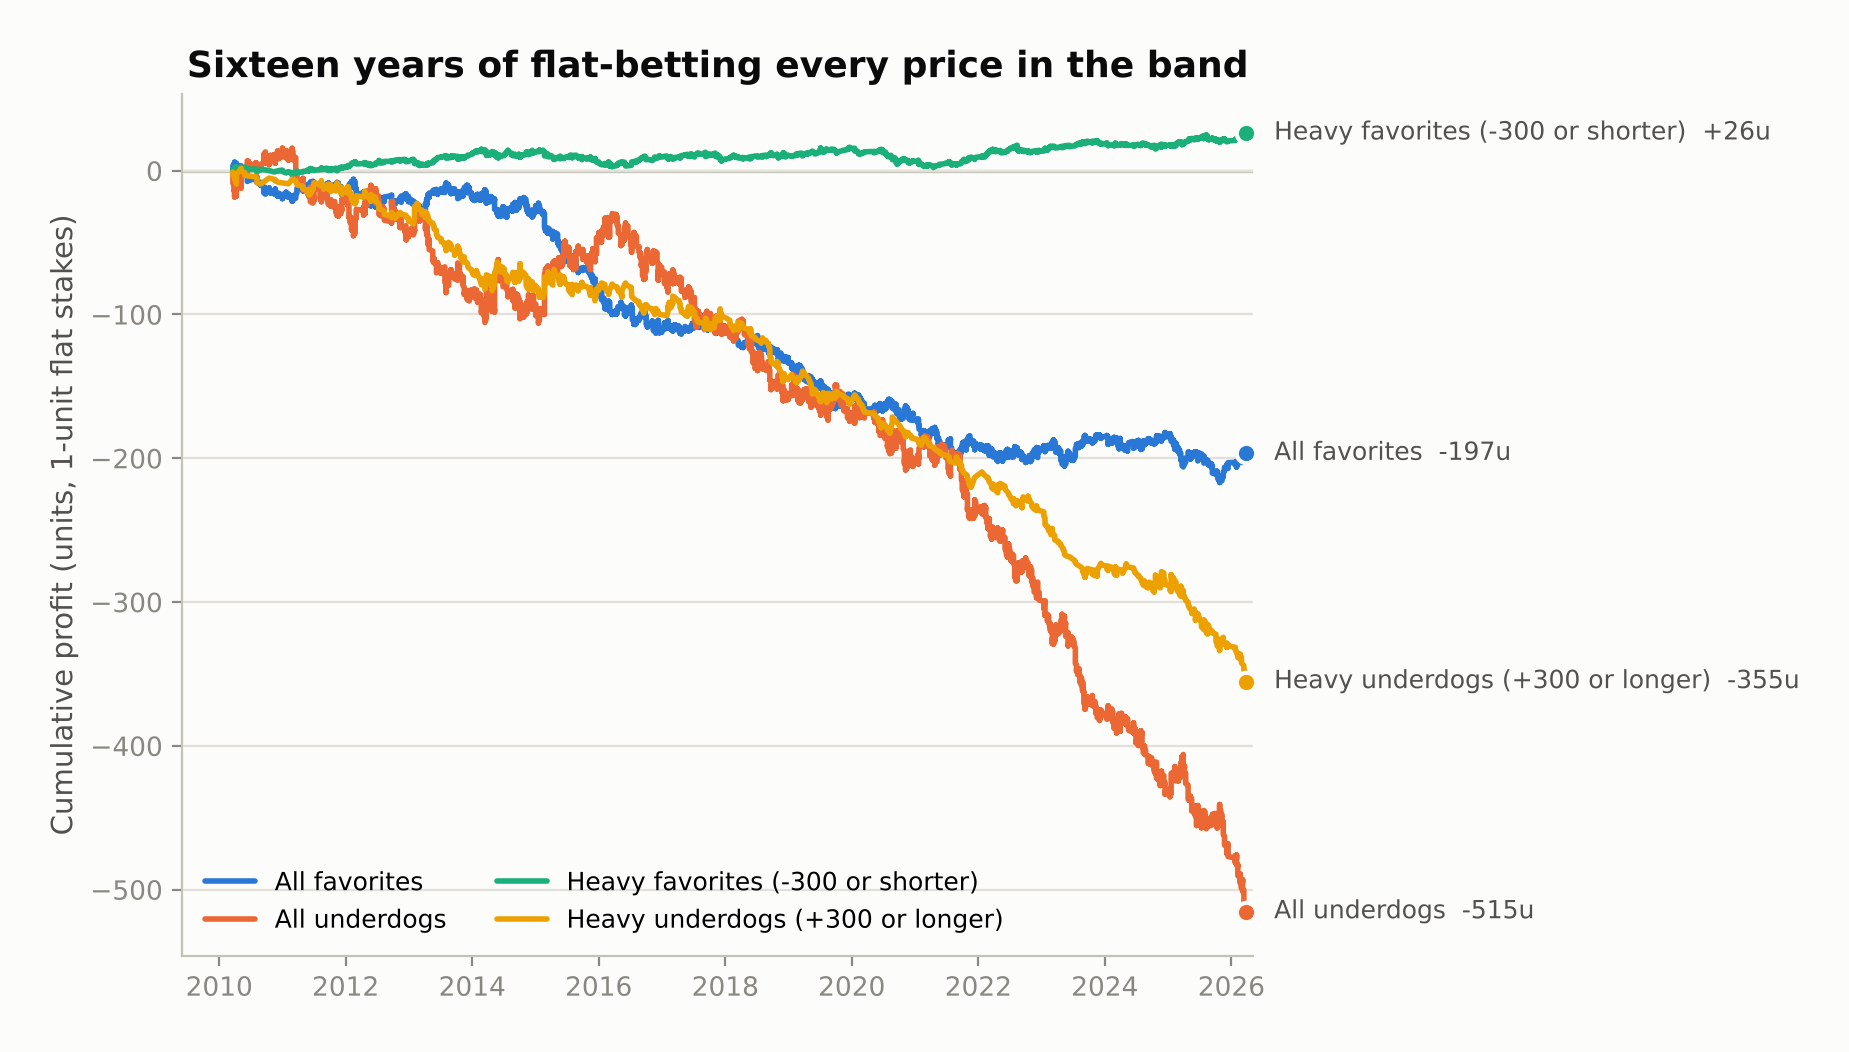
\includegraphics[width=0.9\textwidth]{cumulative_pnl.png}
  \caption{Cumulative profit of 1-unit flat stakes, 2010--2026. Heavy favorites
  ($-300$ or shorter) end $+26$ units through the vig; heavy underdogs ($+300$ or longer) lose
  355 units.}
  \label{fig:pnl}
\end{figure}

\subsection{The bias is not an early-market relic}

Re-estimating the M--Z slope by era gives $1.03$ (SE 0.06) for 2010--2015, $1.11$ (0.06) for
2016--2020, and $1.21$ (0.06) for 2021--2026 --- the latest era rejects efficiency on its own
($p<0.001$), and the point estimates \emph{rise} across eras (Figure~\ref{fig:eras}). Whatever
generates the mispricing has not been competed away; it has grown with the sport's mainstream
(and recreational-bettor) audience, consistent with demand-side accounts of FLB
\citep{snowberg2010} and difficult to reconcile with early-market naivety.

\begin{figure}[t]
  \centering
  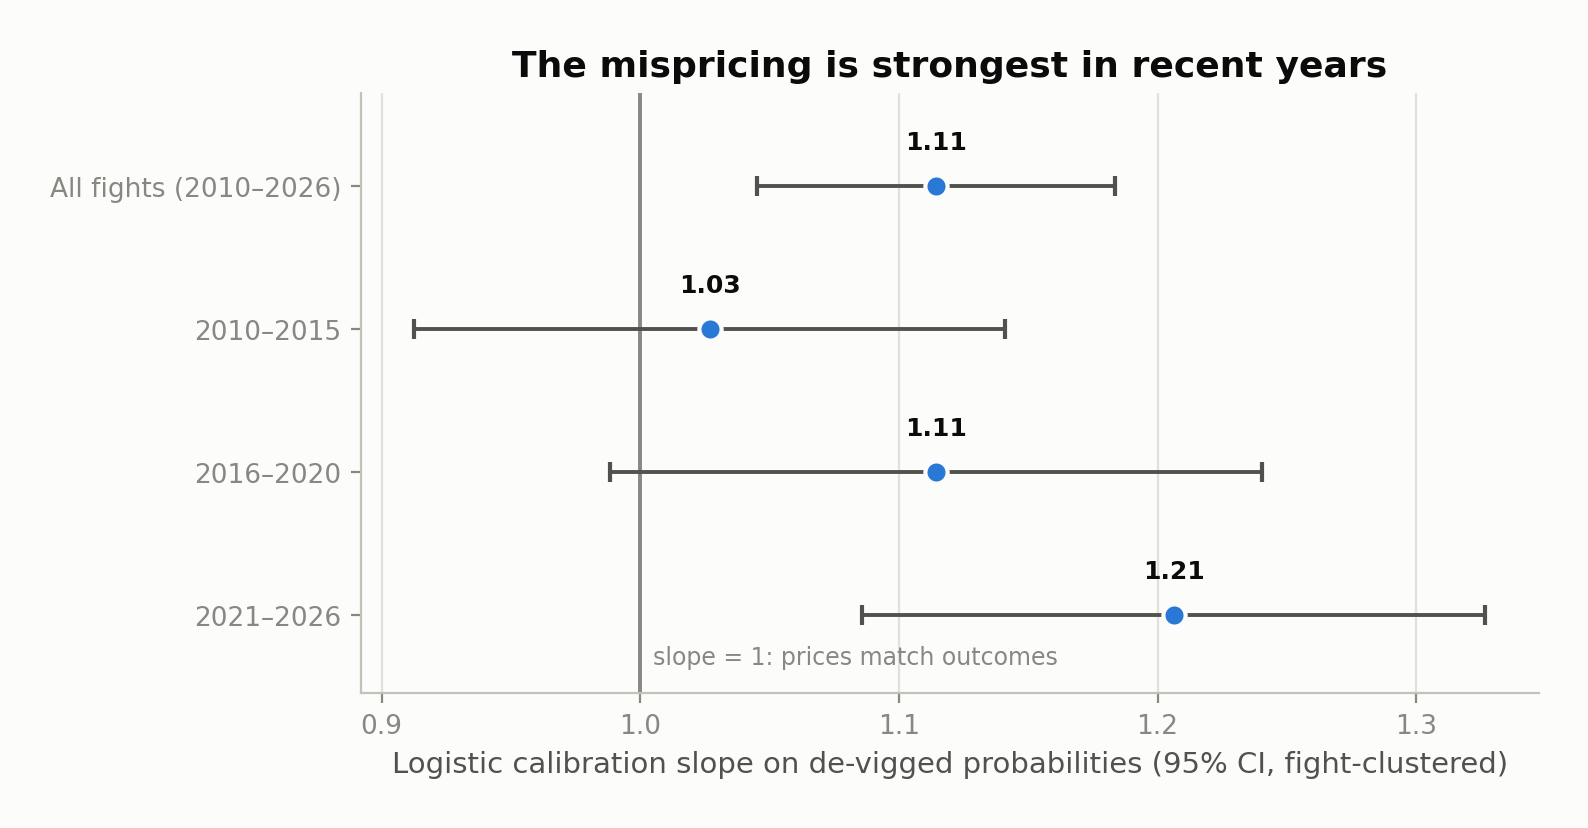
\includegraphics[width=0.85\textwidth]{slope_stability.png}
  \caption{Calibration slope by era with 95\% intervals (fight-clustered). The mispricing is
  strongest in the most recent era.}
  \label{fig:eras}
\end{figure}

\subsection{Semi-strong efficiency: public information cannot beat the line (H3)}

If the tails are mispriced, does the market also ignore public information? No.
Table~\ref{tab:ml} reports the out-of-sample benchmark on 1{,}882 fights from 2022--2026. A
logistic model on 17 public career differentials alone is \emph{much} worse than the market
(log-loss gap $+0.0178$, 95\% CI $[+0.009, +0.027]$). Adding the market probability as a feature
recovers the market almost exactly and improves on it by a statistically indistinguishable
$-0.0027$ $[-0.0075, +0.0021]$; gradient boosting overfits and loses. A betting simulation that
backs whichever side the combined model prices above the raw market price never achieves a
significant ROI at any edge threshold (point estimates $-0.8\%$ to $+1.8\%$, minimum one-sided
$p = 0.40$).
H3 survives: the anomaly is a systematic distortion of tail prices, not exploitable neglect of
public statistics --- mispricing and informational efficiency coexist.

\begin{table}[t]
\centering
\begin{threeparttable}
\caption{Out-of-sample benchmark vs.\ the closing line, 2022--2026 ($n=1{,}882$ fights).}
\label{tab:ml}
\begin{tabular}{lcccc}
\toprule
Model & Log loss & Brier & AUC & $\Delta$ log loss vs.\ market [95\% CI] \\
\midrule
Market (\devig{} odds)          & 0.588 & 0.201 & 0.642 & --- \\
Stats only (logistic)           & 0.606 & 0.208 & 0.583 & $+0.018$ $[+0.009, +0.027]$ \\
Stats $+$ market (logistic)     & 0.585 & 0.201 & 0.645 & $-0.003$ $[-0.008, +0.002]$ \\
Stats $+$ market (grad.\ boost) & 0.599 & 0.207 & 0.632 & $+0.011$ $[+0.001, +0.021]$ \\
\bottomrule
\end{tabular}
\begin{tablenotes}\footnotesize
\item Chronological split (train $\le$ 2021). Negative $\Delta$ = model beats the market. CIs:
paired bootstrap over test fights. Features are favorite-minus-underdog career differentials
computed from per-corner columns; rows oriented favorite-vs-underdog so corner assignment cannot
leak.
\end{tablenotes}
\end{threeparttable}
\end{table}

\subsection{Exploitability at the sportsbook: real bias, marginal profit (H4)}

Bias and exploitability are different claims, and the second demands a stricter test: scanning
sixteen years for the best-looking rule and reporting its return is data snooping. In the
walk-forward protocol, the rule chosen on 2010--2017 alone (by highest bootstrap lower bound ---
the pessimistic criterion) is ``flat-bet every favorite at $-300$ or shorter,'' with training ROI
$+1.0\%$ on 829 bets. Staked blind on 2018--2026 it returned $\mathbf{+1.9\%}$ per bet on 975
bets ($+18.1$ units; 95\% CI $[-1.2, +4.7]$), versus the $-4.0\%$ an efficient market implies for
those prices (Figure~\ref{fig:exploit}). The bias therefore did not evaporate after its
``discovery'' in training data --- the rule beat the efficient-market benchmark by roughly six
points of ROI --- but its profit is not statistically distinguishable from zero (one-sided
$p = 0.11$). At average closing prices, H4 is not rejected: the tradeable content of the anomaly
at a sportsbook is mostly \emph{avoidance} (never flat-bet longshots), not a reliable money pump.

\begin{figure}[t]
  \centering
  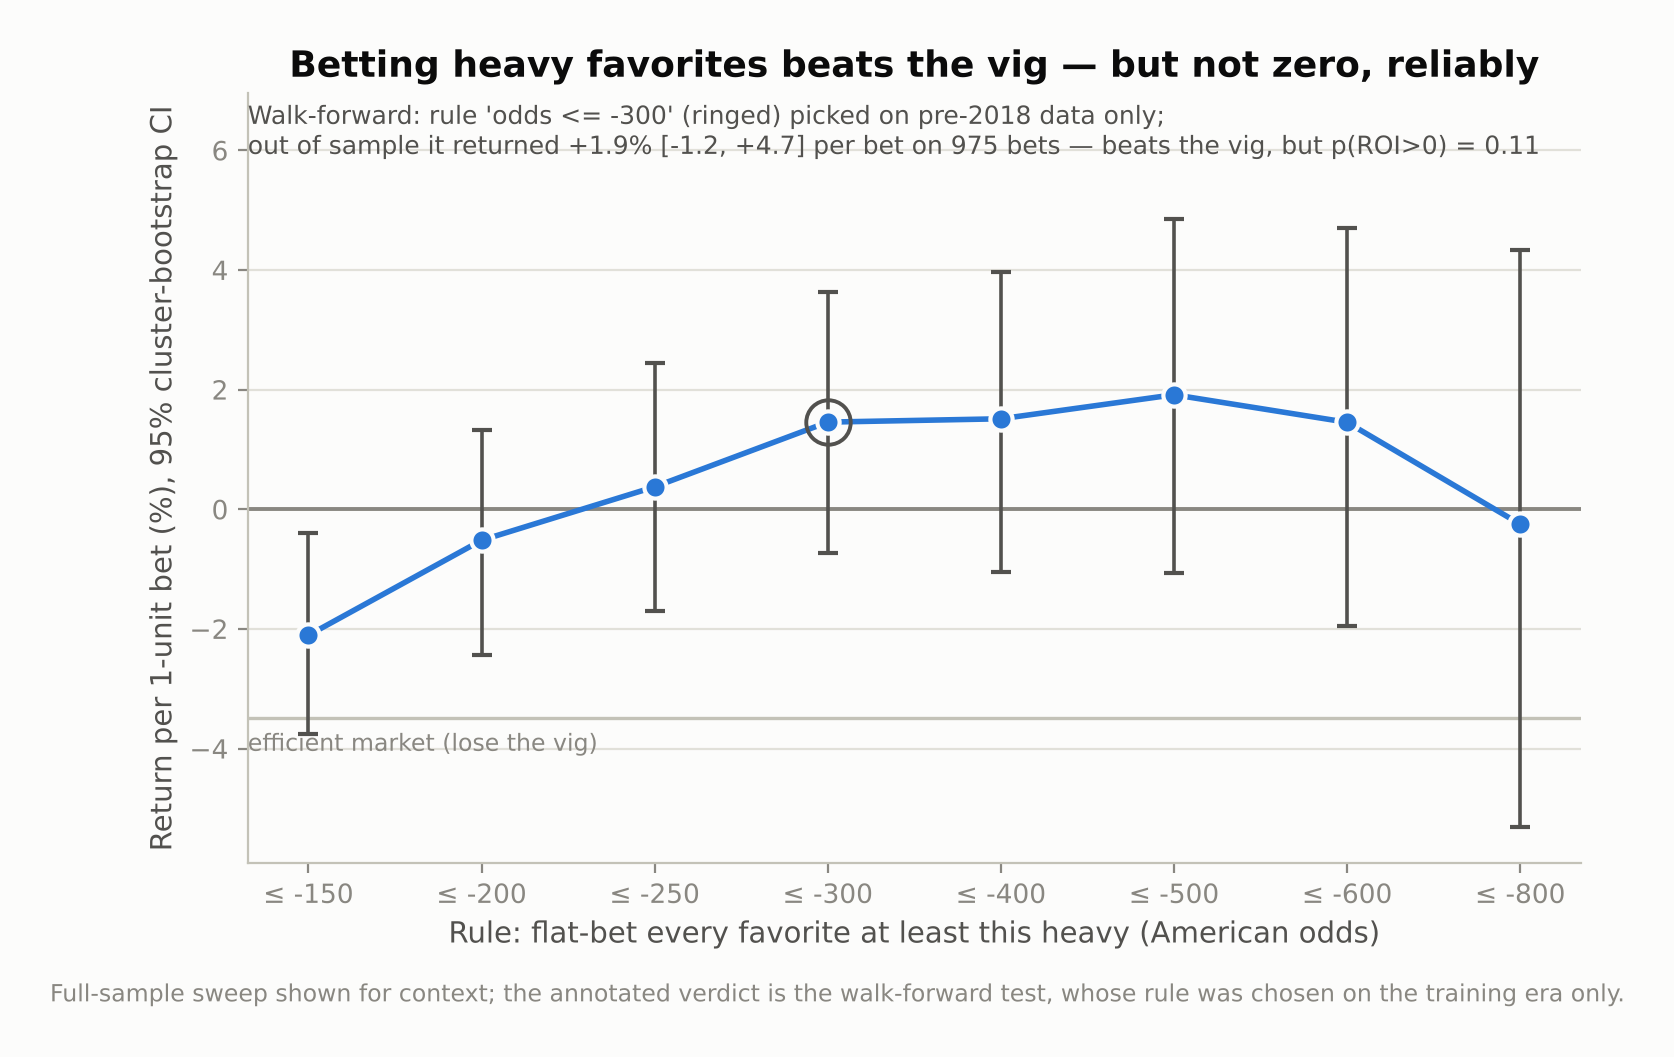
\includegraphics[width=0.9\textwidth]{exploitability.png}
  \caption{Favorite-cutoff sweep (full sample, for context) and the walk-forward verdict. The
  ringed rule was selected on 2010--2017 data only and staked blind on 2018--2026.}
  \label{fig:exploit}
\end{figure}

\subsection{Execution on a prediction market: fees are not the constraint (H5)}
\label{sec:fees}

The preceding test prices execution at a sportsbook, where the friction --- the overround --- is
baked into the price. Event-contract exchanges change the cost structure entirely. On Kalshi, a
YES contract on the favorite trades at a price $P \in (0,1)$ dollars and pays \$1 at settlement;
there is no vig in the price, and the explicit costs are a trading fee and the bid--ask spread.
Kalshi's fee schedule (effective July 7, 2026) charges, per contract and only on execution
(settlement, membership, and ACH transfers are free):
\[
\text{taker fee} = 0.07\,P(1-P), \qquad \text{maker fee} = 0.0175\,P(1-P).
\]
The fee is a parabola peaking at $P=\$0.50$ (1.75 cents). The edge documented in this paper lives
at $P \approx 0.75$--$0.90$, where the taker fee is 0.6--1.3 cents per contract --- as a share of
the price paid, essentially $0.07(1-P)$, i.e.\ $0.7$--$1.8\%$, \emph{falling} in the favorite's
price. The
venue that appears expensive for coin-flip contracts is nearly free precisely where the FLB edge
sits, while the sportsbook's effective margin (${\sim}4\%$ of stake) does not shrink for
favorites.

Kalshi listed its first UFC markets in 2025, so no historical exchange prices exist for this
sample, and H5 cannot be tested against realized exchange quotes. We therefore model execution
under explicit counterfactual price scenarios spanning optimistic to worst-case. Staking \$1 buys
$1/(P + \mathrm{fee})$ contracts; the per-dollar return is $\text{won}/(P+\mathrm{fee}) - 1$.
Under (price $=$ raw closing implied probability, fee $=0$) this accounting reproduces the
sportsbook flat-bet return exactly --- a unit-tested identity, so the scenarios generalize the
baseline rather than changing the measurement.

\begin{table}[t]
\centering
\begin{threeparttable}
\caption{The walk-forward out-of-sample bets (favorites $\le -300$, 2018--2026, $n=975$) under
execution scenarios.}
\label{tab:fees}
\begin{tabular}{lccccc}
\toprule
Scenario & Price basis & Fee (\% of stake) & ROI & 95\% CI & $p$ \\
\midrule
Sportsbook closing line (baseline) & raw close        & ---    & $+1.9\%$ & $[-1.2, +4.7]$ & 0.10 \\
Kalshi taker at the mid            & \devig{} close   & 1.5\%  & $+4.5\%$ & $[+1.4, +7.4]$ & $<0.001$ \\
Kalshi taker, mid $+$ 1\textcent{} & \devig{} $+$ .01 & 1.4\%  & $+3.3\%$ & $[+0.2, +6.1]$ & 0.012 \\
Kalshi taker, mid $+$ 2\textcent{} & \devig{} $+$ .02 & 1.4\%  & $+2.1\%$ & $[-1.0, +4.9]$ & 0.076 \\
Kalshi maker at the mid            & \devig{} close   & 0.4\%  & $+5.7\%$ & $[+2.5, +8.6]$ & $<0.001$ \\
Kalshi taker at book price (worst) & raw close        & 1.3\%  & $+0.6\%$ & $[-2.4, +3.3]$ & 0.35 \\
\bottomrule
\end{tabular}
\begin{tablenotes}\footnotesize
\item Fees per Kalshi's official schedule; exact formula without per-order rounding (rounding
adds at most one cent per order). CIs: fight-cluster bootstrap; $p$: one-sided against
$\mathrm{ROI}\le 0$. Mean prices: raw close \$0.816, \devig{} mid \$0.783. The baseline row
recomputes the Section~4.5 bets inside the cost model's bootstrap; its $p$ of $0.10$ vs.\ $0.11$
there is seed variation at $B=4{,}000$. The maker row ignores fill risk and adverse selection
and is an upper bound.
\end{tablenotes}
\end{threeparttable}
\end{table}

Table~\ref{tab:fees} and Figure~\ref{fig:fees} give the result. If the exchange mid tracks the
\devig{} consensus of the books --- the standard assumption for liquid, arbitrage-linked sports
markets --- the identical bets that were marginal at the book clear zero decisively: $+4.5\%$ per
bet as a taker at the mid ($p < 0.001$), because the ${\sim}4$ points the book kept as vig accrue
to the bettor while the exchange charges only $1.5\%$. The edge survives crossing a one-cent
half-spread ($+3.3\%$, $p = 0.012$), thins at two cents ($+2.1\%$, $p = 0.076$), and disappears
in the worst case where the exchange price embeds the book's full margin ($+0.6\%$, $p = 0.35$).
The full-sample version of the rule (1{,}804 bets, 2010--2026) shows the same ordering (mid
taker $+3.5\%$, $p = 0.002$; one-cent spread $+2.2\%$, $p = 0.022$; two cents $+1.0\%$,
$p = 0.17$), as does the recent era alone (2021--2026, 650 bets: mid taker $+5.8\%$,
$p < 0.001$; even the \emph{sportsbook} baseline is positive there at $+3.0\%$, $p = 0.04$,
though selecting the strongest era after observing it is descriptive, not confirmatory).

A breakeven decomposition makes the economics transparent. Out of sample the favorites won
$83.2\%$ of fights against a mean \devig{} mid of $78.3\%$: an edge of $4.9$ probability points.
Total friction (fee plus effective half-spread) of up to $6.2\%$ of the mid price would be
required to erase it. The Kalshi taker fee consumes $1.5\%$, leaving roughly $3.7$ cents per
contract of headroom for the spread --- several times the tick width quoted on liquid sports
markets. This is why the verdict is insensitive to the fee and hinges entirely on price
formation: \emph{whether} Kalshi's UFC mids actually sit at the \devig{} book consensus, at
book-equivalent prices, or --- if exchange participants correct the bias --- at the true
probability, at which point no venue rescues the strategy. Evidence that prediction markets
exhibit their own favorite--longshot bias \citep{page2013} makes the consensus-tracking scenario
plausible, but only forward collection of exchange quotes can settle it.

\begin{figure}[t]
  \centering
  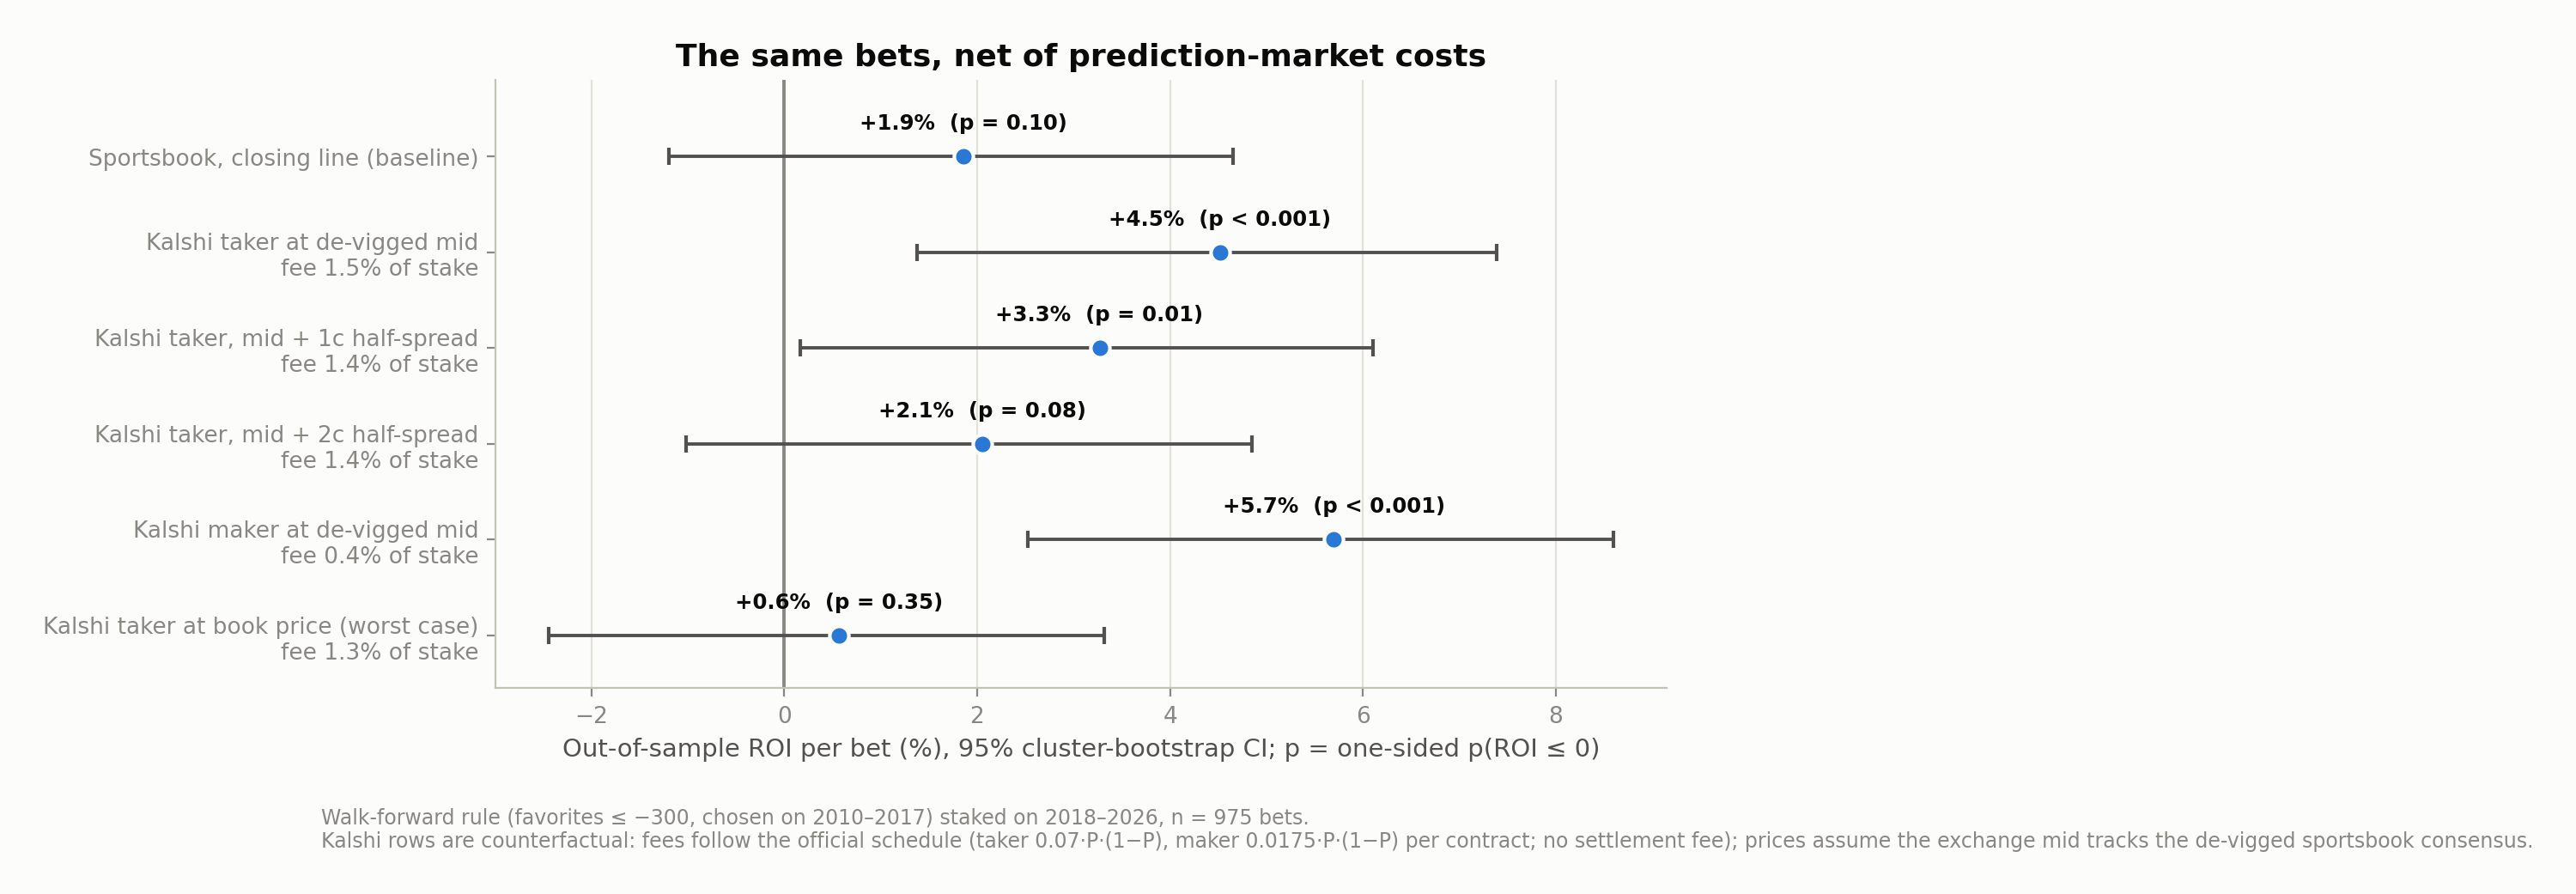
\includegraphics[width=0.95\textwidth]{fees_scenarios.png}
  \caption{Out-of-sample ROI of the walk-forward rule under execution scenarios, with 95\%
  cluster-bootstrap intervals and one-sided $p$-values. Kalshi rows are counterfactual: fees
  follow the official schedule; prices are assumptions about exchange price formation.}
  \label{fig:fees}
\end{figure}

\section{Verification and robustness audit}

Because this study makes an economic claim, the analysis was audited end to end before results
were interpreted. The audit covered five classes of error.

\emph{Reproducibility.} The entire pipeline --- data filters, tests, tables, figures --- runs
from one command with fixed random seeds, and every number in this paper regenerates
bit-identically from the frozen dataset snapshot. The repository ships 27 unit tests covering the
statistical machinery.

\emph{Statistical dependence.} The two sides of a fight are mirror images. Every regression
clusters by fight; every bootstrap resamples whole fights; calibration buckets de-duplicate
mirrored pairs (alternating which side is kept, since always keeping one corner would inject the
corner-assignment effect into the pick'em bucket). The unit tests include power checks on
synthetic markets: a calibrated market ($\beta = 1$) produces no rejection and no walk-forward
edge; a market simulated with $\beta = 1.35$ produces both.

\emph{Vig contamination.} All headline claims are stated on \devig{} probabilities; the bias
survives the conservative Shin correction, whose insider-defense mechanism would otherwise be the
leading supply-side confound. The economic tests use a benchmark ($1/r - 1$) that is
price-invariant under proportional margin, so band comparisons are apples to apples.

\emph{Data snooping.} The exploitability claim rests solely on a rule selected on 2010--2017 by a
pessimistic criterion and evaluated once on 2018--2026. The full-sample sweep and the recent-era
slice are reported as context and labeled descriptive. Per-bucket calibration $p$-values carry
FDR control.

\emph{Look-ahead and leakage in the ML benchmark.} Chronological split; features built only from
pre-fight career columns; fights oriented favorite-vs-underdog so corner labels cannot leak; the
dataset's own pre-computed differential columns (which mix orientations) are not used. The
fee-scenario accounting was validated by an identity test: with price set to the raw close and
zero fee it reproduces the sportsbook return series exactly.

\section{Limitations}

Five limitations bound the conclusions. First, odds are closing lines from a single aggregated
source; intraday movement, best-price line shopping across books, and bet limits are outside the
data. Second, the exchange scenarios are counterfactual: Kalshi listed no UFC markets before
2025, so the mid-tracks-consensus assumption, quoted depth at 80-cent-plus prices, position
limits, and maker fill rates are all untested on this sample --- the maker row in particular is
an upper bound that ignores adverse selection. Third, although the walk-forward protocol
guards against rule snooping, the broader research design (studying favorites because the FLB
literature predicts favorites) is itself informed by prior evidence; the protection is the
out-of-sample era, not ignorance of the hypothesis. Fourth, results are UFC-specific; other
promotions' markets may differ. Fifth, the profitable cell is concentrated: heavy favorites win
$83\%$ of the time, so the strategy's returns are a long series of small gains punctuated by
$-100\%$ losses, and its five-point probability edge is real money only at stake sizes the
historical exchange order books may not have absorbed.

\section{Conclusion}

UFC moneyline markets from 2010--2026 present a sharp two-sided picture. They are informationally
efficient --- superbly calibrated through the middle of the probability range, impounding public
fighter statistics so completely that no model built on them beats the closing line --- and yet
systematically mispriced at the tails, in the classic favorite--longshot direction, by margins
that are economically enormous on the longshot side (a 29-cent-per-dollar flat-bet loss on heavy
underdogs) and statistically decisive throughout (calibration slope $1.114$, $p = 0.001$, robust
to Shin de-vigging, strongest in the most recent era).

On the question this study set out to answer --- \emph{is there an exploitable edge once
prediction-market costs are accounted for?} --- the answer is: \textbf{the costs are not the
obstacle}. At sportsbook closing prices the pre-registered favorites rule beat the
efficient-market benchmark by six points of ROI out of sample but could not clear zero
statistically ($+1.9\%$, $p = 0.11$), because the book's margin consumes most of the mispricing.
Kalshi's fee at heavy-favorite prices is roughly a third of that margin at the sample's mean
price, and settlement is free; under the standard assumption that exchange mids track the \devig{} book consensus, the
same bets return $+4.5\%$ per bet ($p < 0.001$) net of fees, surviving a realistic spread. What
the fee schedule cannot guarantee is the price: if exchange participants price fights at
book-equivalent levels --- or correct the bias entirely --- the edge shrinks to noise. The
binding constraints on exploiting a seventy-year-old anomaly in a modern market are price
formation and depth, not explicit transaction costs. Collecting exchange quotes on UFC markets
going forward, now that they exist, would convert H5 from a scenario analysis into a direct
test, and is the natural next step.

\section*{Reproducibility statement}

All results derive from a pinned snapshot of the public Ultimate UFC Dataset (6{,}904 fights,
2010-03-21 to 2026-03-28) and regenerate bit-identically via \texttt{python run\_analysis.py}
(fixed seeds, $B = 4{,}000$ bootstrap resamples throughout; 27 passing unit tests via
\texttt{pytest}). The repository contains the full pipeline: odds conversion and de-vigging
(proportional, power, Shin), calibration and returns tests, the walk-forward protocol, the ML
benchmark, and the Kalshi fee model (\texttt{src/mma\_efficiency/costs.py}), together with all
tables (\texttt{results/}) and figures (\texttt{figures/}) used here.

\begin{thebibliography}{99}

\bibitem[Ali(1977)]{ali1977}
Ali, M.~M. (1977). Probability and utility estimates for racetrack bettors.
\emph{Journal of Political Economy}, 85(4), 803--815.

\bibitem[Benjamini and Hochberg(1995)]{bh1995}
Benjamini, Y., and Hochberg, Y. (1995). Controlling the false discovery rate: a practical and
powerful approach to multiple testing. \emph{Journal of the Royal Statistical Society B}, 57(1),
289--300.

\bibitem[Griffith(1949)]{griffith1949}
Griffith, R.~M. (1949). Odds adjustments by American horse-race bettors.
\emph{American Journal of Psychology}, 62(2), 290--294.

\bibitem[Kalshi(2026)]{kalshifees}
Kalshi (2026). \emph{Fee schedule}, effective July 7, 2026.
\url{https://kalshi.com/docs/kalshi-fee-schedule.pdf}.

\bibitem[Mincer and Zarnowitz(1969)]{mincer1969}
Mincer, J., and Zarnowitz, V. (1969). The evaluation of economic forecasts. In J.~Mincer (ed.),
\emph{Economic Forecasts and Expectations}, NBER.

\bibitem[Page and Clemen(2013)]{page2013}
Page, L., and Clemen, R.~T. (2013). Do prediction markets produce well-calibrated probability
forecasts? \emph{Economic Journal}, 123(568), 491--513.

\bibitem[Shin(1993)]{shin1993}
Shin, H.~S. (1993). Measuring the incidence of insider trading in a market for state-contingent
claims. \emph{Economic Journal}, 103(420), 1141--1153.

\bibitem[Snowberg and Wolfers(2010)]{snowberg2010}
Snowberg, E., and Wolfers, J. (2010). Explaining the favorite--long shot bias: is it risk-love or
misperceptions? \emph{Journal of Political Economy}, 118(4), 723--746.

\bibitem[\v{S}trumbelj(2014)]{strumbelj2014}
\v{S}trumbelj, E. (2014). On determining probability forecasts from betting odds.
\emph{International Journal of Forecasting}, 30(4), 934--943.

\bibitem[Thaler and Ziemba(1988)]{thaler1988}
Thaler, R.~H., and Ziemba, W.~T. (1988). Anomalies: parimutuel betting markets: racetracks and
lotteries. \emph{Journal of Economic Perspectives}, 2(2), 161--174.

\bibitem[mdabbert(2026)]{ufcdata}
mdabbert. \emph{Ultimate UFC Dataset} (Apache-2.0). Kaggle;
mirror: \url{https://github.com/shortlikeafox/ultimate_ufc_dataset}.

\bibitem[Wolfers and Zitzewitz(2004)]{wolfers2004}
Wolfers, J., and Zitzewitz, E. (2004). Prediction markets.
\emph{Journal of Economic Perspectives}, 18(2), 107--126.

\end{thebibliography}

\end{document}
